

\documentclass[letterpaper, 12pt]{article}

\usepackage{times}
\usepackage{margin}
\usepackage{natbib}
\usepackage{etoolbox}
\usepackage{astjnlabbrev-jh}
\usepackage{bibentry}
\usepackage{ifthen}
\usepackage{epsfig}

% package for copyright symbol
\usepackage{textcomp}

%\usepackage{graphicx}
\usepackage{enumitem}
\usepackage{amssymb, amsmath}
\usepackage{xcolor}
\usepackage{listings}
\usepackage{commath}
\usepackage{rotating}

\usepackage{dirtree}
\usepackage{changepage}

%\usepackage[T1]{fontenc}
%\usepackage[scaled]{beramono}
%\usepackage[utf8]{inputenc}
%\renewcommand*\familydefault{\ttdefault}

% \lstset{
% language=Python,
% showstringspaces=false,
% formfeed=\newpage,
% tabsize=4,
% commentstyle=\itshape,
% basicstyle=\ttfamily,
% morekeywords={models, lambda, forms}
% }
 
% \newcommand{\code}[2]{
% \hrulefill
% \subsection*{#1}
% \lstinputlisting{#2}
% \vspace{2em}
% }

% Default fixed font does not support bold face
\DeclareFixedFont{\ttb}{T1}{txtt}{bx}{n}{10} % for bold
\DeclareFixedFont{\ttm}{T1}{txtt}{m}{n}{10}  % for normal
% twelve-sized ttm:
\DeclareFixedFont{\tttb}{T1}{txtt}{bx}{n}{12}  % for bold
\DeclareFixedFont{\tttm}{T1}{txtt}{m} {n}{12}  % for normal

\DeclareFixedFont{\ttnm}{T1}{txtt}{m}{n}{9.8}  % for normal

% Custom colors
\usepackage{color}
\definecolor{deepblue}  {rgb}{0.0, 0.0, 0.5}
\definecolor{deepred}   {rgb}{0.8, 0.0, 0.0}
\definecolor{deepgreen} {rgb}{0.0, 0.5, 0.0}
\definecolor{commentc}  {rgb}{0.5, 0.5, 0.5}
\definecolor{DodgerBlue}{rgb}{0.1, 0.6, 1.0}

% Python style for highlighting
\newcommand\pythonstyle{\lstset{
language=Python,
basicstyle = \ttm,
morekeywords = {self, as, assert, with, yield}, % Add keywords here
keywordstyle  = \ttb\color{blue},      %
emph        = {MyClass, __init__},     % Custom highlighting
emphstyle   = \ttb\color{DodgerBlue},  % Custom  highlighting style
stringstyle = \color{deepred},         % Strings highlighting style
commentstyle=\color{commentc},         % Comment highlighting style
frame       = tb,                      % Any extra options here
showstringspaces = false
}}

% Python environment:
\lstnewenvironment{python}[1][]{\pythonstyle\lstset{#1}}{}
% Python for external files:
\newcommand\pythonexternal[2][]{{\pythonstyle\lstinputlisting[#1]{#2}}}
% Python for inline:
\newcommand\pythoninline[1]{{\pythonstyle\lstinline!#1!}}

% Copyright
\DeclareTextCommandDefault{\textcopyright}{\textcircled{c}}

% Python style for highlighting
\newcommand\plainstyle{\lstset{
language=Python,
basicstyle = \ttnm,
keywordstyle  = \ttnm,      %
emph        = {MyClass, __init__},     % Custom highlighting
emphstyle   = \ttnm\color{black},    % Custom  highlighting style
stringstyle = \color{black},         % Strings highlighting style
commentstyle=\color{black},         % Comment highlighting style
frame       = tb,                      % Any extra options here
showstringspaces = false
}}

% Plain environment:
\lstnewenvironment{plain}[1][]{\plainstyle\lstset{#1}}{}

\newcommand\plaininline[1]{{\plainstyle\lstinline!#1!}}


%\usepackage{fancyvrb}
%\usepackage{fixltx2e}
%\usepackage{pxfonts}
%\usepackage[tiny,compact]{titlesec}
%\usepackage{bera}
%\usepackage{alltt}
%\renewcommand{\ttdefault}{txtt}

% To use boldface verbatim:
%\lstset{basicstyle=\ttfamily,
%        escapeinside={||},
%        mathescape=true}

\lstset{
    language={[LaTeX]TeX},
    basicstyle=\tt\color{red},
    escapeinside={||},
}

\bibliographystyle{apj_hyperref}
\usepackage[%pdftex,      %%% hyper-references for pdflatex
bookmarks=true,           %%% generate bookmarks ...
bookmarksnumbered=true,   %%% ... with numbers
colorlinks=true,          % links are colored
citecolor=blue,           % green   % color of cite links
linkcolor=blue,           %cyan,         % color of hyperref links
menucolor=blue,           % color of Acrobat Reader menu buttons
urlcolor=blue,            % color of page of \url{...}
breaklinks=true,
linkbordercolor={0 0 1},  %%% blue frames around links
pdfborder={0 0 1},
frenchlinks=true]{hyperref}
%\usepackage{breakurl}

\newcommand{\eprint}[1]{\href{http://arxiv.org/abs/#1}{#1}}
\newcommand{\ISBN}[1]{\href{http://cosmologist.info/ISBN/#1}{ISBN: #1}}
\providecommand{\adsurl}[1]{\href{#1}{ADS}}

% hyper ref only the year in citations:
\makeatletter
% Patch case where name and year are separated by aysep:
\patchcmd{\NAT@citex}
  {\@citea\NAT@hyper@{%
     \NAT@nmfmt{\NAT@nm}%
     \hyper@natlinkbreak{\NAT@aysep\NAT@spacechar}{\@citeb\@extra@b@citeb}%
     \NAT@date}}
  {\@citea\NAT@nmfmt{\NAT@nm}%
   \NAT@aysep\NAT@spacechar\NAT@hyper@{\NAT@date}}{}{}
% Patch case where name and year are separated by opening bracket:
\patchcmd{\NAT@citex}
  {\@citea\NAT@hyper@{%
     \NAT@nmfmt{\NAT@nm}%
     \hyper@natlinkbreak{\NAT@spacechar\NAT@@open\if*#1*\else#1\NAT@spacechar\fi}%
       {\@citeb\@extra@b@citeb}%
     \NAT@date}}
  {\@citea\NAT@nmfmt{\NAT@nm}%
   \NAT@spacechar\NAT@@open\if*#1*\else#1\NAT@spacechar\fi\NAT@hyper@{\NAT@date}}
  {}{}
\makeatother


%\def\bibAnnoteFile#1{}
%\bibpunct[, ]{(}{)}{,}{a}{}{,}

% Packed reference list:
\setlength\bibsep{0pt}

% \textwidth=6.5in
% \textheight=9.5in
% \topmargin=-0.75in
% \oddsidemargin=0.0in
% \evensidemargin=0.0in

% \pagestyle{myheadings}
% \markright{MC\sp{3}}
% \pagenumbering{arabic}


% :::::::::::::::::::::::
\newcommand\degree{\degr}
\newcommand\degrees{\degree}
\newcommand\vs{\emph{vs.}}

% unslanted mu, for ``micro'' abbrev.
\DeclareSymbolFont{UPM}{U}{eur}{m}{n}
\DeclareMathSymbol{\umu}{0}{UPM}{"16}
\let\oldumu=\umu
\renewcommand\umu{\ifmmode\oldumu\else\math{\oldumu}\fi}
\newcommand\micro{\umu}
\newcommand\micron{\micro m}
\newcommand\microns{\micron}

\let\oldsim=\sim
\renewcommand\sim{\ifmmode\oldsim\else\math{\oldsim}\fi}
\let\oldpm=\pm
\renewcommand\pm{\ifmmode\oldpm\else\math{\oldpm}\fi}
\newcommand\by{\ifmmode\times\else\math{\times}\fi}
\newcommand\ttt[1]{10\sp{#1}}
\newcommand\tttt[1]{\by\ttt{#1}}
\newcommand\tablebox[1]{\begin{tabular}[t]{@{}l@{}}#1\end{tabular}}
\newbox{\wdbox}
\renewcommand\c{\setbox\wdbox=\hbox{,}\hspace{\wd\wdbox}}
\renewcommand\i{\setbox\wdbox=\hbox{i}\hspace{\wd\wdbox}}
\newcommand\n{\hspace{0.5em}}
\newcommand\marnote[1]{\marginpar{\raggedright\tiny\ttfamily\baselineskip=9pt #1}}
\newcommand\herenote[1]{{\bfseries #1}\typeout{======================> note on page \arabic{page} <====================}}
\newcommand\fillin{\herenote{fill in}}
\newcommand\fillref{\herenote{ref}}
\newcommand\findme[1]{\herenote{(FINDME: #1)}}

\newcount\timect
\newcount\hourct
\newcount\minct
\newcommand\now{\timect=\time \divide\timect by 60
         \hourct=\timect \multiply\hourct by 60
         \minct=\time \advance\minct by -\hourct
         \number\timect:\ifnum \minct < 10 0\fi\number\minct}

\newcommand\citeauthyear[1]{\citeauthor{#1} \citeyear{#1}}

\newcommand\mc{\multicolumn}
\newcommand\mctc{\multicolumn{2}{c}}


% {\tttm -h, --help} \\
% Print the list of arguments. \newline

% \newenvironment{myindentpar}[1]%
%   {\begin{list}{}%
%          {\setlength{\leftmargin}{3cm}}%
%      \item[]%
%   }
% {\end{list}}

\newenvironment{packed_enum}{
\begin{enumerate}[leftmargin=3cm]
   \setlength{\itemsep}{1pt}
   \setlength{\parskip}{5pt}
   \setlength{\parsep}{0pt}
}{\end{enumerate}}

\newcommand{\argument}[2]{{\noindent\tttm #1}%
\begin{adjustwidth}{2.5em}{0pt}%
#2 \vspace{0.3cm}%
\end{adjustwidth}%
}

%\newcommand{\ttmb}[1]{\tttm\color{#1}}
\newcommand{\routine}[2]{{\noindent\tttm\color{blue} #1:}%
\begin{adjustwidth}{2.0em}{0pt}%
#2 \vspace{0.15cm}%
\end{adjustwidth}%
}

% \newcommand{\routine}[2]{{\noindent\tttm\color{blue} #1}%
% \begin{adjustwidth}{0.0em}{0pt}%
%  #2 \vspace{0.15cm}%
% \end{adjustwidth}%
% }

% :::::::::::::::::: jhmacs2.tex :::::::::::::::::::::::::::::::::::::
\typeout{Joe Harrington's personal setup, Wed Jun 17 10:53:17 EDT 1998}
% Tue Mar 29 22:23:03 EST 1994

% :::::: pato.tex ::::::
% Joetex character unreservations.
% This file frees most of TeX's reserved characters, and provides
% several alternatives for their functions.


% utility
\catcode`@=11

% comments are first....
\newcommand\comment[1]{}

\newcommand\commenton{\catcode`\%=14}
\newcommand\commentoff{\catcode`\%=12}

% Not-a-comment:
\newcommand\nocomment[1]{#1}

\renewcommand\math[1]{$#1$}
\newcommand\mathshifton{\catcode`\$=3}
\newcommand\mathshiftoff{\catcode`\$=12}

\comment{alignment tab}
\let\atab=&
\newcommand\atabon{\catcode`\&=4}
\newcommand\ataboff{\catcode`\&=12}

\let\oldmsp=\sp
\let\oldmsb=\sb
\def\sp#1{\ifmmode
           \oldmsp{#1}%
         \else\strut\raise.85ex\hbox{\scriptsize #1}\fi}
\def\sb#1{\ifmmode
           \oldmsb{#1}%
         \else\strut\raise-.54ex\hbox{\scriptsize #1}\fi}
\newbox\@sp
\newbox\@sb
\def\sbp#1#2{\ifmmode%
           \oldmsb{#1}\oldmsp{#2}%
         \else
           \setbox\@sb=\hbox{\sb{#1}}%
           \setbox\@sp=\hbox{\sp{#2}}%
           \rlap{\copy\@sb}\copy\@sp
           \ifdim \wd\@sb >\wd\@sp
             \hskip -\wd\@sp \hskip \wd\@sb
           \fi
        \fi}
\def\msp#1{\ifmmode
           \oldmsp{#1}
         \else \math{\oldmsp{#1}}\fi}
\def\msb#1{\ifmmode
           \oldmsb{#1}
         \else \math{\oldmsb{#1}}\fi}
\def\supon{\catcode`\^=7}
\def\supoff{\catcode`\^=12}
\def\subon{\catcode`\_=8}
\def\suboff{\catcode`\_=12}
\def\supsubon{\supon \subon}
\def\supsuboff{\supoff \suboff}


\newcommand\actcharon{\catcode`\~=13}
\newcommand\actcharoff{\catcode`\~=12}

\newcommand\paramon{\catcode`\#=6}
\newcommand\paramoff{\catcode`\#=12}

\comment{And now to turn us totally on and off...}

\newcommand\reservedcharson{ \commenton  \mathshifton  \atabon  \supsubon
                             \actcharon  \paramon}

\newcommand\reservedcharsoff{\commentoff \mathshiftoff \ataboff \supsuboff
                             \actcharoff \paramoff}

\newcommand\nojoe[1]{\reservedcharson #1 \reservedcharsoff}

\catcode`@=12
\reservedcharsoff

\reservedcharson
\newcommand\jhauth[1]{{#1}}
\newcommand\jhstud[1]{{#1}}

\comment{Must have ONLY ONE of these... trust these macros, they work
\newcommand\jhauth[1]{{\bfseries #1}}
\newcommand\jhstud[1]{{\em #1}}
}

\reservedcharsoff
\reservedcharson


% ::::::::::::::::::::::::::::::::::::::::::::::::::::

\def\vs{{\em vs.}}
\def\p{\phantom{(0)}}

% Section levels:
\setcounter{secnumdepth}{5}
%  \section{}       % level 1
%  \subsection{}    % level 2
%  \subsubsection{} % level 3
%  \paragraph{}     % level 4 - equivalent to subsubsubsection
%  \subparagraph{}  % level 5

% To show in the table of content:
\setcounter{tocdepth}{5}

% Linebreak after \paragraph
\makeatletter
\renewcommand\paragraph{%
   \@startsection{paragraph}{4}{0mm}%
      {-\baselineskip}%
      {.5\baselineskip}%
      {\normalfont\normalsize\bfseries}}
\makeatother

% Linebreak after \paragraph
\makeatletter
\renewcommand\subparagraph{%
   \@startsection{subparagraph}{4}{0mm}%
      {-\baselineskip}%
      {.5\baselineskip}%
      {\normalfont\normalsize\bfseries}}
\makeatother

\actcharon
\renewcommand{\textfraction}{0.1}
\comment{\paramon\def\herenote#1{}\paramoff}
\renewcommand{\thepage}{\arabic{page}}
\reservedcharson

% :::::::::::: My Additions ::::::::::::::
\newcommand\Spitzer{{\em Spitzer}}
\newcommand\SST{{\em Spitzer Space Telescope}}
\newcommand\chisq{$\chi^2$}
\newcommand\itbf[1]{\textit{\textbf{#1}}}
\newcommand\bftt[1]{\texttt{\textbf{#1}}}
\newcommand\function[1]{\noindent\texttt{\begin{tabular}{@{}l@{}l}#1\end{tabular}}\newline}
\newcommand\bfv[1]{|\textbf{#1}|}
\newcommand\ttred[1]{\textcolor{red}{\ttfamily #1}}
\newcommand\ttblue[1]{\textcolor{blue}{\ttfamily #1}}
\newcommand\ttblack[1]{\textcolor{black}{\ttfamily #1}}
\newcommand\der{{\rm d}}
\newcommand\tno{$\sp{-1}$}
\newcommand\tnt{$\sp{-2}$}
\newcommand*\Eval[3]{\left.#1\right\rvert_{#2}^{#3}}
\newcommand\mcc{MC\sp{3}}
\newcommand\transit{{\tt Transit}}
\newcommand\pylineread{{\tttm Pylineread}}
%:::::::::::::::::::::::::::::::::::::::::
% Next six lines adjust spacing above/below captions and Sections etc
% Adjust as needed

\comment{
% \setlength{\abovecaptionskip}{0pt}
% \setlength{\belowcaptionskip}{0pt}
% \setlength{\textfloatsep}{8pt}
% \titlespacing{\section}{0pt}{5pt}{*0}
% \titlespacing{\subsection}{0pt}{5pt}{*0}
% \titlespacing{\subsubsection}{0pt}{5pt}{*0}
}

\reservedcharsoff
\actcharon
\mathshifton

\reservedcharson

\usepackage{epsfig}
\textwidth=6.5in
\textheight=9.5in
\topmargin=-0.75in
\oddsidemargin=0.0in
\evensidemargin=0.0in

\pagestyle{myheadings}



\markright{{\bf TEA Code Description, Blecic \& Bowman}}
\pagenumbering{arabic}
  
\begin{document}

\begin{titlepage}
\begin{center}

% Title
\textsc{\huge \bfseries TEA}\\[0.5cm]
\textsc{\LARGE Thermochemical Equilibrium Abundances}\\[0.5cm]
\rule{250pt}{0.4pt} \\[0.4cm]
{ \huge \bfseries Code Description\\[0.4cm] }

\rule{250pt}{0.4pt} \\[1cm]

% Author and supervisor
\begin{minipage}{0.4\textwidth}
\begin{flushleft} \large
\emph{Authors:}\\
 \textsc{Jasmina Blecic \\M.~Oliver Bowman}
\end{flushleft}
\end{minipage}
\begin{minipage}{0.4\textwidth}
\begin{flushright} \large
\emph{Programmers: } \\
\textsc{M.~Oliver Bowman Jasmina Blecic }
\end{flushright}
\end{minipage}\\[1.5cm]


\begin{minipage}{0.4\textwidth}
\begin{flushleft} \large
\emph{Lead Scientist:}\\
 \textsc{Jasmina Blecic}
\end{flushleft}
\end{minipage}
\begin{minipage}{0.4\textwidth}
\begin{flushright} \large
\emph{Principal Investigator:} \\
\textsc{Joseph Harrington}
\end{flushright}
\end{minipage}\\[.5cm]

\vfill

% Bottom of the page
{\large \today}

\end{center}
\end{titlepage}


% Copyright page

\vspace*{\fill}
\begin{center}
\begin{minipage}{.8\textwidth}


\vspace{20pt} This document goes along with the TEA code, the TEA theory
paper \citep{BlecicEtal2016-TEAtheory}, and the code description
document.  \\

 TEA is part of the PhD dissertation work of Dr. Jasmina                   
Blecic, who developed it with coding assistance from                       
undergraduate M. Oliver Bowman and under the advice of                     
Prof. Joseph Harrington at the University of Central Florida,              
Orlando, Florida, USA.   \\      

\hspace{60pt} Copyright \textcopyright \hspace{1pt} 2014-2016 University of Central Florida. \\   

This program is reproducible-research software: you can                    
redistribute it and/or modify it under the terms of the                    
Reproducible Research Software License as published by                     
Prof. Joseph Harrington at the University of Central Florida,              
either version 0.3 of the License, or (at your option) any later           
version.  \\   
                                                             
This program is distributed in the hope that it will be useful,            
but WITHOUT ANY WARRANTY; without even the implied warranty of             
MERCHANTABILITY or FITNESS FOR A PARTICULAR PURPOSE.  See the              
Reproducible Research Software License for more details.  \\                 

You should have received a copy of the Reproducible Research               
Software License along with this program.  If not, see                     
{\tt http://planets.ucf.edu/resources/reproducible/}.  The license's           
preamble explains the situation, concepts, and reasons surrounding         
reproducible research, and answers some common questions.  \\                

This project was started with the support of the NASA Earth and            
Space Science Fellowship Program, grant NNX12AL83H, held by                
Jasmina Blecic, Principal Investigator Joseph Harrington, and the          
NASA Science Mission Directorate’s Planetary Atmospheres Program,          
grant NNX12AI69G.     \\                                                     
                                                                           
See the file ACKNOWLEDGING in the top-level TEA directory for              
instructions on how to acknowledge TEA in publications.  \\                  
                                                                           
We welcome your feedback, but do not guarantee support.                    
Many questions are answered in the TEA forums:   \\                          
                                                                          
{\tt https://physics.ucf.edu/mailman/listinfo/tea-user}                          
{\tt https://physics.ucf.edu/mailman/listinfo/tea-devel}   \\                      
                                                                           
Visit our Github site:                               
{\tt https://github.com/dzesmin/TEA/}   \\                                         
                                                                           
Reach us directly at:                                                      
\\ Jasmina Blecic: jasmina@physics.ucf.edu 
\\ Joseph Harrington: jh@physics.ucf.edu \\                                     

\end{minipage}
\end{center}
\vfill % equivalent to \vspace{\fill}


% Table of contents
\tableofcontents
\newpage
\section{Code Overview}

The Thermochemical Equilibrium Abundances (TEA) package
(Figure \ref{fig:TEAflow}) is composed of five different types of
programs: {\bf Library Programs} that read thermodynamic libraries and
collect stoichiometric information, {\bf TEA Drivers} that execute TEA
for a single $T, P$ point or a list of multiple $T, P$ points, {\bf
Main Science Programs} that perform the iterative Lagrange
minimization technique and Lambda correction algorithm, {\bf File
Control Programs} that manage input-output files and operations, and
{\bf Auxiliary Programs} that help the user to make proper input and
plot the TEA output.




\begin{figure}[!h]
    \centering
    \includegraphics[width=12.25cm, trim=22 100 27 110,
    clip=true]{figs/TEAFlow.ps}
    \includegraphics[width=11cm, trim=22 340 27 320,
    clip=true]{figs/LegFlow.ps}
\caption{Layout of the pre-pipeline and pipeline packages.}
\label{fig:TEAflow}
\end{figure}




  The code is built in a modular fashion where each that program
  performs calculations can be easily controlled by a driver program
  or be otherwise replaced as long as the appropriate inputs and
  outputs are conserved.  This modular work-flow facilitates strict
  control over what calculations are performed and where, and allows
  future users easy access to code manipulations or additions.  As the
  TEA code is an open-source package, such modifications are
  encouraged if the user wishes to fine-tune any mechanics or apply
  new techniques in order to reach equilibrium abundances.
  
This is a third part of a three-part document describing the TEA
code. The first part, the TEA theory
document \citep{BlecicEtal2016-TEAtheory}, presents the theoretical
basis for the method applied, the second part is a user manual, and
this document contains programs description to allow the user future
modifications. If you find this package useful for your research,
please cite \citet{BlecicEtal2016-TEAtheory}.


  This project was completed with the support of the NASA Earth and
  Space Science Fellowship Program, grant NNX12AL83H, held by Jasmina
  Blecic, PI Joseph Harrington. Project development included graduate
  student Jasmina Blecic and undergraduate M. Oliver Bowman.



\section{Code Description}

This text is divided into five sections, each describing the
aforementioned types of programs with detailed descriptions of each
routine.

\subsection{Library Programs}
\label{PrepipeSec}

The TEA {\bf Library Programs} read the thermodynamic tables and the
elemental abundances file to store the necessary thermochemical data
and stoichiometric information in TEA readable files. These files are
further used by the TEA {\bf Driver programs} and {\bf Main Scientific
Programs}. These library programs consist of three
modules: \texttt{prepipe.py}, \texttt{readJANAF.py}
and \newline \texttt{makestoich.py}. Currently, these modules process
the JANAF tables and the elemental abundances file made based on
Asplund et al. (2009), both provided with the code. The user can feed
the code with their own library granted the format that TEA can
process is obeyed.

These programs are executed prior to the release, and the
thermochemical data and stoichiometric information needed for TEA to
run are provided with the code. However, if updated JANAF tables are
obtained, a pre-pipeline execution will populate the files with new
information.


\subsubsection{prepipe.py}

This program sets and/or executes the pre-pipeline TEA
routines \texttt{readJANAF.py} and \newline \texttt{makestoich.py}. It
consists of two functions: \texttt{comp()} and \texttt{setup()}. The
\texttt{comp()} function counts the number of each element in a
 chemical species, while the \texttt{setup()} function reads the JANAF
tables and allows sharing of common routines for \texttt{readJANAF.py}
and \texttt{makestoich.py}. If executed as \texttt{prepipe.py}, it
will run both routines. The user can also run each routine separately,
if desired.

The \texttt{comp()} function is the species-counting function. It
counts the number of each element in a chemical species by taking in a
string of a chemical species (i.e., "H2O") and returning an array
containing every element with corresponding counts found in that
species. It is called by \texttt{makestoich.py} and
the \texttt{setup()} function. The user can also return a
stoichiometric array containing only the elements found in the input
species. Otherwise, it returns the full array of all 113 available
elemental stoichiometric data.

The \texttt{setup()}routine reads raw JANAF tables placed in the
appropriate directory (default: \texttt{janaf/}) and extracts
thermodynamic and stoichiometric data of interest. It serves as a
setup for the \texttt{readJANAF.py} and \texttt{makestoich.py}
routines. The program takes the names of the raw JANAF tables
directory, thermodynamic output directory, stoichiometric output
directory, output stoichiometric file, and the pre-written file
containing abundance data \newline
(default: \texttt{abundances.txt}). It takes number of elements
from \texttt{comp()} and loops over all JANAF data and abundance data,
performing various thermodynamic calculations and stoichiometric
functions on the appropriate species of interest.


\subsubsection{makestoich.py}

This code makes the \texttt{stoich\_out} file
(default: \texttt{stoich.txt}) that carries stoichiometric values of
all species that appear in the JANAF tables. It reads the chemical
formula from each JANAF file to obtain the number of atomic weights of
each element in each species. Also reads in bulk elemental abundances
from \texttt{abundances.txt} that currently uses Asplund et al. (2009)
solar photosphere abundances. The code creates a temporary directory
where JANAF tables are converted into stoichiometric tables. The
tables carry a unique name and state, given by the top line in each
JANAF table: (i.e., original JANAF table \texttt{Al-001.txt} is
converted to \texttt{Al\_ref.txt}).  If desired, user can preserve
this directory (in \texttt{TEA.cfg}, doprint = \texttt{True}).

The names of the files in the temporary directory have the following
format: {
\begin{enumerate}
\setlength\itemsep{0ex}
\setlength\topsep{0ex}
\setlength\partopsep{0ex}
\setlength\parsep{0ex}

   \item If a species appears just once in JANAF tables, it gets the
   unique name of the compound and its state and is defined
   as \texttt{originals} in the code
   (example: \texttt{CH4\_$\sb{g}$}).  \item If a species appears
   several times, it is defined as \texttt{redundant} in the code and
   an additional string is added to differentiate among them
   (example: \texttt{Al2O3\_{cr}\_{Alpha}, \newline
   Al2O3\_{cr}\_{Beta}, Al2O3\_{cr}\_{Kappa}}). This is defined by the
   isomer name in the JANAF tables.
\end{enumerate}


The setup of this code is done in \texttt{prepipe.py}
inside \texttt{setup()}. The code retrieves the setup information,
creates a temporary directory to store the converted files, allocates
space for these files with the unique naming scheme described above,
then loops over all JANAF tables to write stoichiometric files.

To write the \texttt{stoich\_{out}} file
(default: \texttt{stoich.txt}), it again loops over all elements
(listed in \texttt{comp()} inside \texttt{prepipe.py}) and matches
them with the abundance data from the abundance file (default:
\texttt{abundances.txt}). If a match is not found, the abundance is set to
zero. This information is written at the top of
the \texttt{stoich\_{out}} file.

For each element in \texttt{comp()} and species in the JANAF tables,
the species name and stoichiometric values are written into
the \texttt{stoich\_{out}} file. The code ignores redundant compounds
as they carry the same stoichiometric values.

The \texttt{prepipe.py} code can execute this code together with
the \texttt{readJANAF.py}. \newline
\texttt{makestoich.py} can also be executed on its own with the simple
 command: \texttt{makestoich.py}. 

}

\subsubsection{readJANAF.py}

This code makes the \texttt{thermo\_dir}
(default: \texttt{/lib/gdata}) directory that carries converted JANAF
tables with only the data needed for TEA to run, namely the
temperature, $T$ in (K), free energy
function \math{(-[G\sp{o}-H\sp{o}(T\sb{r})]/T)} in (J/K/mol), and the
heat of formation \math{(\Delta\sb{f}H\sp{o}}), in (kJ/mol). This
program will remove intermittent commentary in the JANAF files and
will produce separate files for stoichiometrically identical species
with unique descriptors. Output data files are produced in the
format \texttt{/lib/gdata/SPECIES\_STATE.txt}.  The code also
makes \texttt{conversion\_record.txt} that gives the names of the
original, raw JANAF files and the new names given by
\newline \texttt{readJANAF.py}. To sort the file list in
alphabetical order, execute in terminal: \newline \texttt{sort
conversion\_record.txt $>$ conversion\_record\_sorted.txt}

The names of the files have the following format:
{
\begin{enumerate}
\setlength\itemsep{0ex}
\setlength\topsep{0ex}
\setlength\partopsep{0ex}
\setlength\parsep{0ex}

   \item Each converted file carries a unique name and state given by
   the top line in each JANAF file.  \item If a species appears just
   once in JANAF tables, it gets a unique name of the compound and its
   state and is defined as \texttt{originals} in the code
   (example: \texttt{CH4\_$\sb{g}$}).  \item If a species appears
   several times, it is defined as \texttt{redundant} in the code and
   an additional string is added to differentiate among them \newline
   (example: \texttt{Al2O3\_cr\_Alpha, Al2O3\_cr\_Beta,
   Al2O3\_cr\_Kappa}).  \item If a species is an ion, additional
   string is added (example: \texttt{Al-007.txt and Al-008.txt became
   Al\_ion\_n\_g, Al\_ion\_p\_g})
\end{enumerate}
}

The setup of this code is done in \texttt{prepipe.py} inside
the \texttt{setup()} function.The code retrieves pre-pipeline setup
information, creates a directory for converted thermodynamic files,
checks whether a species is redundant in JANAF tables, and
creates \texttt{conversion\_record.txt}. If a species is redundant, an
additional string is added to the file name. The module loops over all
JANAF tables and writes data into the correct columns with the correct
labels.

The \texttt{prepipe.py} code can execute this code together with
the \texttt{readJANAF.py}. \newline
\texttt{readJANAF.py} can also be executed on its own with the simple command: 
\texttt{readJANAF.py}. 


%%%%%%%%%%%%%%%%%%% PIPELINE DRIVERS %%%%%%%%%%%%%%%%%%%%%%%%%%%%%%%%

\subsection{TEA Drivers}

TEA is executed by one of two drivers, depending on if a
single \math{T, P} point or a list of \math{T, P} points are
provided. Both drivers follow the same general flow of execution.

\subsubsection{runsingle.py}
\label{runsingleSec}

This program runs TEA over an input file that contains only one ${T,
P}$ point. The code retrieves the input file and the current directory
name given by the user and sets the locations of all necessary modules
and directories that will be used. It then executes the modules in the
following order: \texttt{makeheader.py}, \texttt{balance,py},
and \texttt{iterate.py}. The final results along with the input and
the configuration files are saved in the {em results/} directory.

This module prints the code progress on screen: the current ${T, P}$
line from the pre-atmosphere file, the current iteration number, and
when the minimization is complete.  \newline Example: \texttt{100
Maximum iteration reached, ending minimization}.

The program is executed with in-shell inputs:\newline
\texttt{runsingle.py <input file> <name of the result directory>}\newline
Example: \texttt{runsingle.py inputs/Examples/inp\_Example.txt
Single\_Example}


\subsubsection{runatm.py}
\label{runatmSec}

This program runs TEA over a pre-atmosphere file that contains
multiple ${T,P}$ points.  The code first retrieves the pre-atmosphere
file and the current directory name given by the user. It then sets
the locations of all necessary modules and directories of files that
will be used. It allocates an array to store the final abundances for
each species of each $T, P$ run. The program loops over all lines
(${T, P}$'s) in the pre-atmosphere file and executes the modules in
the following order: \texttt{readatm.py, makeheader.py, balance,py,
iterate.py}, and \texttt{readoutput.py}. \texttt{Iterate.py}
executes \texttt{lagrange.py}
and \texttt{lambdacorr.py}. \texttt{readoutput.py} reads results from
the TEA iteration loop executed in \texttt{iterate.py}. The abundances
are calculated and stored in an abundance array. The code then opens
the final atmosphere file to write the results. It takes first common
lines from the pre-atmosphere file and writes the data from the stored
radii, temperature, pressure and abundances array. The code has a
condition to save or delete all intermediate files, time stamps for
checking the speed of execution, and is verbose for debugging
purposes. If these files are saved, the function will create a unique
directory for each ${T, P}$ point. This functionality is controlled in
the TEA config file. The final results, along with the input and the
configuration files are saved in the \texttt{results/} directory.

This module prints on screen the current ${T, P}$ line from the
pre-atmosphere file, the current iteration number, and informs the
user that minimization is done.  Example: \texttt{5 100 Maximum
iteration reached, ending minimization}.

The program is executed with in-shell inputs:\newline
\texttt{runatm.py <pre-atmosphere file> <name of the result directory>}\newline
Example: \texttt{runatm.py inputs/Examples/atm\_Example.atm
Atm\_Example}


%%%%%%%%%%%%%%%%%%% MAIN PIPELINE %%%%%%%%%%%%%%%%%%%%%%%%%%%%%%%%

\subsection{Main Scientific Programs}

These programs perform scientific calculations explained in Sections
2, 3, and 4 of \citet{BlecicEtal2016-TEAtheory}. The mass balance
equation, Lagrange optimization system of equations, Lambda correction
procedure, and iterative minimization approach are separated into four
modules,
respectively: \texttt{balance.py}, \texttt{lagrange.py}, \texttt{lambdacorr.py},
and \texttt{iterate.py}. Inclusion of condensates or solids can be
easily implemented inside these modules by modifying the equations
listed in the code comments.

\subsubsection{balance.py}

This code produces an initial guess for the first TEA iteration by
fulfilling the mass balance condition, $\sum\sb{i=1}^n a\sb{ij}\,
x\sb{i} = b\sb{j}$ (equation (17)
in \citealp{BlecicEtal2016-TEAtheory}), where $i$ is species index,
$j$ is element index, $a$'s are stoichiometric coefficients, and $b$'s
are elemental fractions by number, i.e., ratio of number densities of
element '$j$' to the total number densities of all elements in the
system (see the end of Section 2
of \citealp{BlecicEtal2016-TEAtheory}).  The code writes the result
into machine- and human-readable files.

The code begins by making a directory for the output results. It, then
reads the header file and imports all relevant chemical data from it.
To satisfy the mass balance equation, some $y\_i$ variables remain as
free parameters. The number of free parameters is set to the number of
total elements in the system, thus ensuring that the mass balance
equation can be solved for any number of input elements and output
species the user chooses. The code locates a chunk of species ($y\_i$)
containing a sum of $ai\_j$ values that forbids ignoring any element
in the system (sum of the $ai\_j$ values in a column must not be
zero). This chunk is used as a set of free variables in the
system. The initial scale for other $y\_i$ variables is set to a
known, arbitrary number. Starting values for the known species are set
to 0.1 moles, and the mass balance equation is calculated. If this
value does not produce all positive mole numbers, the code
automatically sets known parameters to 10 times smaller and tries
again. Actual mole numbers for the initial guesses of $y\_i$ are
arbitrary, as TEA only requires a balanced starting point to
initialize minimization. The goal of this code is to find a positive
and a non-zero set of mole numbers to satisfy this
requirement. Finally, the code calculates $\bar{y}$, initializes the
iteration number, $\Delta$, and $\bar{\Delta}$ to zero and writes
results into machine- and human-readable output files.

This code is called by \texttt {runatm.py} and \texttt {runsingle.py}
and can be executed alone with in-shell input: \texttt
{balance.py} \texttt{<HEADER\_FILE> <DIRECTORY\_NAME>}



\subsubsection{lagrange.py}

This code applies Lagrange's method and calculates minima based on the
methodology elaborated in Section 3
of \citet{BlecicEtal2016-TEAtheory}. Equations in this code contain
both references and an explicitly written definitions.  The program
reads the last iteration's output and data from the last header file,
creates variables for the Lagrange equations, sets up the Lagrange
equations, and calculates final $x_i$ mole numbers for the current
iteration cycle. Note that the mole numbers that result from this
function are allowed to be negative. If negatives are returned, lambda
correction by
\texttt{lambdacorr.py} is necessary. The final $x_i$ values, as well as 
$\bar{x}$, $\bar{y}$, $\Delta$, and $\bar\Delta$ are written into
machine- and human-readable output files. This function is
executed \texttt{iterate.py} and can be run independently.


\subsubsection{lambdacorr.py}

This module applies lambda correction method described in Section 4
of \citealp{BlecicEtal2016-TEAtheory}). When input mole numbers are
negative, the code corrects them to positive values and pass them to
the next iteration cycle. The code reads the values from the last
\texttt{lagrange.py} output and header file, performs
checks, then starts setting basic equations. It sets a smart range so
it can efficiently explore the lambda values from [0,1]. Half of the
range is sampled exponentially, and the other half linearly, totalling
150 points. The code retrieves the last lambda value before first
derivative becomes positive (equation (34) in TEA theory document),
and corrects negative mole numbers to positive.

The code works without adjustments and with high precision for the
fractional abundances (mixing fractions) up to 10$\sp{-14}$ and the
temperature range of 1000 - 4000 K. For temperatures below 1000 K and
mixing fractions below 10$\sp{-14}$, the code produces results with
low precision. To improve the precision, adjust the lambda exploration
variables \texttt{lower} and \texttt{steps} to larger magnitudes
(i.e., \texttt{lower} = -100, \texttt{steps} = 1000). This will
lengthen the time of execution.

This function is executed \texttt{iterate.py} and can be run
independently.

\subsubsection{iterate.py}

This program executes the iteration loop for TEA. It repeats
Lagrangian minimization \newline (\texttt{lagrange.py}) and lambda
correction (\texttt{lambdacorr.py}) until the maximum iteration is
reached. The code has time stamps for checking the speed of execution
and is verbose for debugging purposes; both are defined
in \texttt{TEA.cfg} file.

The flow of the code goes as follows: the current header, output, and
result directory are read; physical properties are retrieved from the
header, then the \texttt{balance.py} output is read as the initial
iteration input and passed to \texttt{lagrange.py}. Lagrange $x\_i$
values are then checked for negative values; the next iteration starts
either with lambda correction output (if negative $x\_i$'s are found)
or with the output produced by \texttt{lagrange.py} (if all $x\_i$'s
are positive). This procedure is repeated until the maximum iteration
is reached, which stops the loop. Intermediate results from each
iteration step are written in the machine- and human-readable output
files on the user's request in \texttt{TEA.cfg}.

This program is executed by \texttt{runatm.py} and can be executed
alone with in-shell input: \\
\texttt{iterate.py $<$header file$>$ $<$name of the result directory$>$}


%%%%%%%%%%%%%%%%%%% ANCILLARY PROGRAMS %%%%%%%%%%%%%%%%%%%%%%%%%%%%%%%%

\subsection{File Control Programs} 

These programs generate inputs for the {\bf Main Scientific
Programs}, manage reading and processing the input information, and
produce machine- and human-readable output files.

\subsubsection{format.py}

This module allows each program to read the output of the previous
step so the data can be used in the next step. It also manages the
format for each output file and produces both machine- and
human-readable files.

It contains the following functions: 
{
\begin{enumerate}
\setlength\itemsep{0ex}
\setlength\topsep{0ex}
\setlength\partopsep{0ex}
\setlength\parsep{0ex}
   \item {\bf readheader()}: This function reads the current header
   file (one $T, P$) and returns data common to each step of TEA. It
   searches only for the required chemical data from the header file
   and fills out the output arrays appropriately. The function is used
   by \texttt{balance.py, lagrange.py, lambdacorr.py},
   and \texttt{iterate.py}.  \item {\bf readoutput()}: This function
   reads output files made by \texttt{balance.py, \newline
   lagrange.py} and \texttt{lambdacorr.py}. It reads any iteration's
   output and returns the data in an array.  \item {\bf output()}:
   This function produces machine-readable output files. The files are
   saved only if \texttt{saveout = True} in \texttt{TEA.cfg} file. The
   function is used by the \texttt{balance.py, lagrange.py},
   and \texttt{lambdacorr.py}. The function writes the name of the
   header, current iteration number, species list, starting mole
   numbers of species for current iteration, final mole numbers of
   molecular species after the iteration is done, difference between
   starting and final mole numbers, total sum of initial mole numbers,
   total sum of final mole numbers and the change in total mole
   numbers of all species.  \item {\bf fancyout()}: This function
   produces human-readable output files. The files are saved only
   if \texttt{saveout = True} in \texttt{TEA.cfg} file. The function
   is used by \texttt{balance.py},\newline \texttt{lagrange.py},
   and \texttt{lambdacorr.py}. The function writes the name of the
   header, current iteration number, species list, starting mole
   numbers of species for current iteration, final mole numbers of
   molecular species after the iteration is done, difference between
   starting and final mole numbers, total sum of initial mole numbers,
   total sum of final mole numbers, and the change in total mole
   numbers of all species.  If \texttt{doprint = True}, all data
   written to the file is presented on-screen in the same
   human-readable format.  \item {\bf fancyout\_results()}: This
   function produces the final result output for each $T, P$ in the
   human-readable format. The final mole number for each species is
   divided by the total mole numbers of all species in the
   mixture. This gives the mole fraction abundance for each species,
   which are TEA final results. This function is called by
   the \texttt{iterate.py} module.  \item {\bf printout()}: Prints
   iteration progress number or other information in one line of
   terminal.
\end{enumerate}
}


\subsubsection{makeheader.py}
\label{makeheaderSec}

This module contains functions to write headers containing all
necessary chemical data for a single TEA execution using a single $T,
P$ and multiple $T, P$ points. It consists of two main
functions, \newline \texttt{make\_singleheader()}
and \texttt{make\_atmheader()}, both of which are called by the
\newline \texttt{runsingle.py} and \texttt{runatm.py} modules,
respectively. \texttt{header\_setup()}, \newline \texttt{atm\_headarr()}, \texttt{single\_headarr()},and \texttt{write\_header()}
are supporting functions for these main functions. This module is
imported by \texttt{runatm.py} and \texttt{runsingle.py} to create the
header files.

{\bf header\_setup()} - This function is a common setup for both
single $T, P$ and multiple $T, P$ runs of TEA. Given the
thermochemical data and stoichiometric table, this function returns
stoichiometric values and an array of chemical potentials for the
species of interest at the current temperature and pressure.  Using
the data provided in the JANAF tables and the equations (10) and (11)
from \citet{BlecicEtal2016-TEAtheory}, it calculates the free energies
(chemical potentials) of each species at a certain temperature. It
also returns an array of booleans that marks which information should
be read from \texttt{stoich\_file} for the current species. It is
executed by the \texttt{make\_atmheader()}
and \texttt{make\_singleheader()} functions.

{\bf single\_headarr()} - This function gathers data needed for TEA to
run in a single $T, P$ case. These are: elemental abundances, species
names, and their stoichiometric values. For the list of elements and
species used, it takes the abundances and stoichiometric values and
puts them in the final array. It converts logarithmic (dex) elemental
abundances into number densities. This function is run
by \texttt{make\_singleheader()} and is dependent on results
from \texttt{header\_setup()}.

{\bf atm\_headarr()} - This function gathers data needed for TEA to
run in a multiple $T, P$ case. These are: elemental abundances,
species names, and their stoichiometric values. For the list of
elements and species used, it takes the abundances and stoichiometric
values and puts them in the final array. This function is run
by \texttt{make\_atmheader()} and is dependent on results
from \texttt{header\_setup()}.

{\bf write\_header()} - This function writes a header file that
contains all necessary data for TEA to run. It is called
by \texttt{make\_atmheader()} and \texttt{make\_singleheader()}.

{\bf make\_singleheader()} - This is the main function that creates a
header for a single $T, P$ run of TEA. It reads the input $T, P$ file
and retrieves necessary data. It then calls
the \texttt{header\_setup()}, \newline \texttt{single\_headarr()},
and \texttt{write\_header()} functions to create a header for the
single $T, P$ point. This function is called by
the \texttt{runsingle.py} module.

{\bf make\_atmheader()} - This is the main function that creates a TEA
header for one $T, P$ of a pre-atmosphere file. It retrieves number of
elements and species used for only the $q$-th $T, P$ point in the
pre-atmosphere file. It then calls
the \texttt{header\_setup()}, \texttt{atm\_headarr()},
and \texttt{write\_header()} functions to create a header for this
point. This function is called by the \texttt{runatm.py} module.
    



\subsubsection{readatm.py}

This function reads a pre-atmosphere file and returns the data that
TEA will use.  It opens a pre-atmosphere file to find markers for
species and TEA data, retrieves the species list, reads data below the
markers, and fills out data into corresponding arrays. It also returns
number of runs TEA must execute for each $T, P$. The function is used
by \texttt{runatm.py}.


\subsubsection{readconf.py}

This code reads the TEA config file, \texttt{TEA.cfg}. There are two
sections in \texttt{TEA.cfg}: the 'TEA' section and the 'PRE-ATM'
section. The 'TEA' section carries parameters and booleans to run and
debug TEA, whereas 'PRE-ATM' section carries parameters to make a
pre-atmospheric file (see Section \ref{makeatm}).




%%%%%%%%%%%%%%%%%%% AUXILIARY PROGRAMS %%%%%%%%%%%%%%%%%%%%%%%%%%%%%%%%

\subsection{Auxiliary Programs}

These programs are provided for the user's convenience. They allow for
the easy generation of the multiple ${T, P}$ pre-atmosphere files
(input for the \texttt{runatm.py} module), and for plotting the
desired abundances profile from the final multiple ${T, P}$ atmosphere
files (output of the \texttt{runatm.py} module).


\subsubsection{makeatm.py}
\label{makeatm}

This module produces a pre-atmosphere file in the format that TEA can
read. Before running \texttt {makeatm.py}, the \texttt {TEA.cfg} file
needs to be edited with the following information: location of the
$PT$ file, the desired name of the pre-atmosphere file, desired input
elemental species, and desired output molecular species.

To run the code type in the terminal: \texttt {makeatm.py
$<$DIRECTORY\_NAME$>$}. \newline The \texttt{$<$DIRECTORY\_NAME$>$} is
the name of the directory where the user wants the current run to be
placed. The pre-atmopshere file will be placed in \texttt
atm\_inputs\} under the \newline \texttt{$<$DIRECTORY\_NAME$>$}
directory.

This module consists of 2 functions:
{
\begin{enumerate}
\setlength\itemsep{0ex}
\setlength\topsep{0ex}
\setlength\partopsep{0ex}
\setlength\parsep{0ex}

   \item {\bf readPT()} - reads the pressure-temperature profile from
   the PT file provided. If custom made, it must be in the format
   provided in the \texttt {doc/examples/} directory.  \item {\bf
   makeatm()} - produces a pre-atmosphere file in the format that TEA
   can read. The file will be placed in the \texttt {atm\_inputs/}
   directory. It calls \texttt {readPT()} to get the pressure and
   temperature array and reads the elemental abundance data file
   (default: \texttt
   {abundances.txt}, \citet{AsplundEtal2009-SunAbundances}). The code
   trims the abundance data to the elements of interest, converts
   species dex abundances into number densities and divides them by
   the hydrogen number densities fractional abundances. It writes data
   (pressure, temperature, elemental abundances) into a
   pre-atmospheric file. The configuration, pressure and temperature,
   and abundances files are copied to the \texttt {atm\_inputs/}
   directory.
\end{enumerate}
}




\subsubsection{plotTEA.py}
This code plots a figure of temperature vs. abundances for the final
atmosphere file produced by TEA. It needs 2 arguments on the command
line: the path to the atmosphere file name and the names of the
species user wants to plot.

Arguments given should be in the following format: {
\begin{enumerate}
\setlength\itemsep{0ex}
\setlength\topsep{0ex}
\setlength\partopsep{0ex}
\setlength\parsep{0ex}

   \item {\bf filename} - string. Full path to the atmospheric
   file.  \item {\bf species} - list of strings. List of species that
   user wants to plot. Species names should be given with their
   symbols (without their states) and no breaks between species names
   (e.g., \texttt{CH4,CO,H2O}).
\end{enumerate}
}

To run the code execute: \texttt{plotTEA.py $<$RESULT\_ATM\_FILE$>$
$<$SPECIES\_NAMES$>$} \\ Example: \texttt{plotTEA.py
results/atm\_Example/atm\_Example.atm
CO,CH$\sb{4}$,H$\sb{2}$O,NH$\sb{3}$} The plot is opened once execution
is completed and saved in the \texttt{plots/} directory.


{\footnotesize
\bibliography{TEA-Manual}
}


\actcharon
\mathshifton

\pagebreak
\end{document}

\end{document}
















